\chapter{Algorithmes variationnels quantiques}
\label{cha:algorithmes-variationnels-quantiques}
%-----------------------------------------------------------------------------%

En général, le comptage est un problème ardu. En acceptant une solution approximative, la complexité de ce problème peut être déplacée à l'échantillonnage quasi uniforme de solutions grâce à l'algorithme de JVV. Toutefois, la construction d'un tel générateur n'a pas encore été évoquée. En fait, la majorité des solveurs de problèmes \textsf{\#P} ne se basent pas sur l'échantillonnage en raison de la difficulté d'obtenir une distribution uniforme composée de solutions. Est-ce que le calcul quantique peut offrir une méthode efficace pour la génération uniforme de solutions?

Les \textit{algorithmes variationnels quantiques} (« Variational Quantum Algorithms ») (VQA) sont des algorithmes hybrides, c'est-à-dire composés d'une partie quantique et d'une partie classique, conçus pour exploiter les avantages du calcul quantique tout en profitant de la puissance des algorithmes classiques~\cite{cerezoVariationalQuantumAlgorithms2021}. Ces algorithmes ont émergé comme la stratégie dominante pour atteindre l'avantage quantique avec le matériel informatique quantique actuel, connu sous le nom des ordinateurs quantiques bruités de taille intermédiaire (« Noisy Intermediate-Scale Quantum ») (NISQ). En effet, les algorithmes quantiques possédant un avantage par rapport aux algorithmes classiques sont actuellement hors d'atteinte pour les ordinateurs quantiques du moment en raison de la taille des systèmes nécessaires et des erreurs causées par le bruit. Les VQA s'inspirent des méthodes d'apprentissage automatique pour résoudre des problèmes d'optimisation combinatoire avec des circuits de faible profondeur sans se soucier de la correction des erreurs des qubits. Un état quantique initial facile à préparer est évolué unitairement avec un circuit quantique paramétré et la valeur moyenne d'une fonction de coût est estimée par de multiples mesures du circuit dans une base appropriée. Les paramètres du circuit sont alors ajustés itérativement par un optimiseur classique afin de minimiser la fonction de coût et ainsi préparer un état près d'une superposition des solutions du problème. Cette approche limite les inconvénients causés par le bruit en raison de l'utilisation de circuits paramétrés limitant la taille des circuits utilisés. La superposition des solutions préparée par les VQA peut être utilisée pour la composante d'échantillonnage de l'algorithme de JVV, améliorant potentiellement les méthodes de comptage basées sur l'échantillonnage.

Parmi les algorithmes englobés par les VQA se place le célèbre \textit{algorithme quantique d'optimisation approximative} (« Quantum Approximate Optimization Algorithm ») (QAOA)~\cite{farhiQuantumApproximateOptimization2014}. Étant l'un des premiers VQA appliqués aux problèmes d'optimisation combinatoire, cet algorithme se prête particulièrement bien à nos demandes. De plus, un grand nombre de travaux ont caractérisé celui-ci en profondeur, facilitant ainsi son application à la question directrice du travail de ce mémoire. Cet algorithme est conséquemment l'objet principal de ce chapitre. 

L'algorithme adiabatique quantique, le fondement théorique de QAOA, est d'abord introduit à la section~\ref{sec:algorithme-adiabatique-quantique}. Après avoir décrit en détail QAOA à la section~\ref{sec:algorithme-quantique-d'optimisation-approximative}, différentes variantes de QAOA sont explorées, telles sa généralisation à l'ansatz quantique à opérateurs alternants et une variante de ce dernier employant le forçage de Grover à la section~\ref{sec:ansatz-quantique-a-operateurs-alternants}. Finalement, deux propriétés de QAOA sont explorées, c'est-à-dire l'initialisation et l'optimisation des paramètres du circuit quantique à la section~\ref{subsec:configuration-des-parametres} et le biais d'échantillonnage à la section~\ref{sec:echantillonnage-et-biais}.

%-----------------------------------------------------------------------------%

\section{Algorithme adiabatique quantique}
\label{sec:algorithme-adiabatique-quantique}

Le \textit{théorème adiabatique}, introduit par Born et Fock~\cite{bornBeweisAdiabatensatzes1928}, peut être énoncé simplement comme suit:

\begin{subtheorem}{Théorème adiabatique}{theoreme-adiabatique}
    Un système physique demeure dans son état propre instantané si une perturbation donnée agit sur lui suffisamment lentement et s'il y a un intervalle significatif entre la valeur propre et le reste du spectre de l'hamiltonien.
\end{subtheorem}

Bien que différentes versions de ce théorème furent rigoureusement formulées~\cite{albashAdiabaticQuantumComputation2018}, une version approximative de celui-ci, proposée par Messiah~\cite{messiahQuantumMechanics1961} et rectifiée par Amin~\cite{aminConsistencyAdiabaticTheorem2009}, est présentée ici dans l'objectif d'élucider les mécanismes du théorème. Un système quantique, décrit par un hamiltonien dépendant du temps $H(t)$, évolue selon l'équation de Schrödinger
\begin{equation}
    i \hbar \frac{\partial \ket{\psi(t)}}{\partial t} = H(t) \ket{\psi} \,.
 \end{equation}
Considérons ici que l'hamiltonien $H(t)$ peut s'écrire sous la forme $H(t) = \tilde{H}(s)$, où $s=t/T \in [0,1]$ est le temps adimensionnel, de manière que $T$ contrôle le taux de variation dans le temps de $H(t)$. Soit $\ket{\varepsilon_{j} (s)}$ les états propres instantanés (potentiellement dégénérés) de $\tilde{H}(s)$ avec énergie $\varepsilon_{j}$ tels que
\begin{equation}
   \tilde{H}(s) \ket{\varepsilon_{j}(s)} = \varepsilon_{j}(s) \ket{\varepsilon_{j}(s)} \,,
\end{equation}
où $\varepsilon_{j}(s) < \varepsilon_{j+1}(s) \ \forall j,s$ et $j \in \set{ 0, 1, 2, \dots }$. L'approximation adiabatique indique qu'un état initial préparé dans un des états propres instantanés $\ket{\varepsilon_{j}(0)}$ demeure dans le même état propre instantané $\ket{\varepsilon_{j}(t)}$ à une phase globale près, à condition que $\varepsilon_{i}(s) - \varepsilon_{j}(s) \neq  0$ et
\begin{equation}
    \label{eq:critere-approximation-adiabatique}
    T \gg \max_{s \in [0,1]} \frac{\lvert \braket{ \varepsilon_{i}(s) | \partial_{s} \tilde{H}(s) | \varepsilon_{j}(s) } \rvert }{\lvert \varepsilon_{i}(s) - \varepsilon_{j}(s) \rvert^{2} } \ \forall j \neq i \,.
\end{equation}
L'approximation adiabatique est souvent utilisée à partir de l'état fondamental $\ket{\varepsilon_{0}(t)}$, menant à la définition du gap spectral entre l'état fondamental et le premier état excité du système $\Delta(s) = \varepsilon_{1}(s) - \varepsilon_{0}(s)$. Généralement, le maximum de $\braket{ \varepsilon_{i}(s) | \partial_{s} \tilde{H}(s) | \varepsilon_{j}(s)}$ est de l'ordre d'une valeur propre typique de $\tilde{H}$ et petit. Ainsi, l'équation~\ref{eq:critere-approximation-adiabatique} indique que le minimum du carré de l'inverse du gap spectral $\Delta$ constitue un critère pratique pour quantifier le temps nécessaire à l'évolution adiabatique.

L'\textit{algorithme adiabatique quantique} (« Quantum Adiabatic Algorithm ») (QAA), introduit par Farhi, Gutmann et Sipser~\cite{farhiQuantumComputationAdiabatic2000}, emploie un ordinateur quantique physique pour la résolution de problèmes d'optimisation combinatoire en se basant sur le théorème adiabatique quantique. Pour ce faire, le système physique est initialement préparé dans l'état fondamental d'un hamiltonien de forçage $H_{D}$ facile à construire et dont l'état fondamental est simple à trouver. La solution du problème, encodée dans l'état fondamental de l'hamiltonien de problème $H_{P}$, est alors obtenue en transitionnant de l'état fondamental de l'hamiltonien $H_{D}$ à l'état fondamental de l'hamiltonien $H_{P}$ par une évolution adiabatique. Plus précisément, l'hamiltonien du système s'écrit comme
\begin{equation}
\label{eq:chemin-adiabatique}    
    \tilde{H}(s) = \left(1-s\right) H_{D} + s H_{P} \,.
\end{equation}
Ainsi, en présumant que le gap spectral entre l'état fondamental et l'état excité est non nul, la solution du problème est toujours obtenue à partir de l'état fondamental final si l'évolution, donnée par l'opérateur $U(t) = e^{-i \int_{0}^{1} \tilde{H}(s) ds}$, est suffisamment lente comme garanti par le théorème adiabatique quantique. Si le temps d'évolution est trop court, une \textit{transition diabatique}, c'est-à-dire une transition de l'état fondamental à un état excité, peut empêcher l'évolution adiabatique.

Typiquement, le gap spectral est non nul~\cite{farhiQuantumComputationAdiabatic2000}, mais cela ne suffit pas à garantir l'efficacité de l'algorithme. En effet, le gap doit suffisamment important pour limiter le temps d'évolution. Pour certains problèmes, cette condition est remplie, permettant une évolution adiabatique en un temps réaliste, mais ce n'est pas toujours le cas~\cite{altshulerAndersonLocalizationMakes2010}. Une alternative consiste à trouver un compromis entre le temps d'évolution et la proximité de l'état final avec l'état fondamental espéré. Le choix du chemin adiabatique utilisé pour transitionner de $H_{D}$ à $H_{P}$ peut aussi différer de l'équation~\ref{eq:chemin-adiabatique}, ce qui peut contribuer à maximiser le gap au long du chemin et donc minimiser le temps d'évolution~\cite{nishimoriExponentialEnhancementEfficiency2017, hormoziNonstoquasticHamiltoniansQuantum2017}.

L'algorithme adiabatique quantique se place au sein du \textit{calcul adiabatique quantique}, qui regroupe différentes méthodes similaires. Un autre membre de ce groupe, le \textit{recuit quantique}, représente généralement l'emploi de QAA dans un environnement bruité, menant ainsi à une version plus réaliste sans contrainte d'adiabaticité ou d'universalité. Cet algorithme partage plusieurs similitudes avec l'algorithme quantique d'optimisation approximative qui seront explorées dans les prochaines sections. 

%-----------------------------------------------------------------------------%

\section{Algorithme quantique d'optimisation approximative}
\label{sec:algorithme-quantique-d'optimisation-approximative}

Bien que le calcul adiabatique quantique puisse être utilisé pour résoudre certains problèmes d'optimisation combinatoire, le temps nécessaire à une évolution adiabatique constitue un facteur limitant pour de nombreux problèmes. L'\textit{algorithme quantique d'optimisation approximative} (« Quantum Approximate Optimization Algorithm ») (QAOA)~\cite{farhiQuantumApproximateOptimization2014} propose alors une alternative, sous la forme d'un algorithme variationnel quantique, discrétisant l'évolution continue de QAA. Cette approche s'éloigne de l'évolution adiabatique en acceptant la présence de transitions diabatiques entre l'état fondamental et les états excités pour réduire le temps d'évolution. L'optimisation des paramètres du circuit quantique paramétré permet de naviguer efficacement l'espace de Hilbert pour atteindre une bonne solution approximative. QAOA est non seulement adiabatique, mais aussi contre-adiabatique, c'est-à-dire qu'il mène à un raccourci à l'adiabacité. En effet, l'erreur de discrétisation peut étonnamment réduire l'impact des excitations diabatiques~\cite{wurtzCounterdiabaticityQuantumApproximate2022}.

%-----------------------------------------------------------------------------

\subsection{Description de l'algorithme}
\label{subsec:description-algorithme}

Étant une idée prometteuse pour les applications des ordinateurs quantiques, l'algorithme quantique d'optimisation approximative a mené à une quantité incroyable de travaux dans les précédentes années~\cite{zhouQuantumApproximateOptimization2020, blekosReviewQuantumApproximate2024}. Ainsi, pour simplifier la compréhension de ce concept, l'algorithme original, dû à Farhi, Goldstone et Gutmann~\cite{farhiQuantumApproximateOptimization2014}, est d'abord présenté.

QAOA repose sur deux différents hamiltoniens: l'hamiltonien de problème, ou de phase, $H_{P}$ et l'hamiltonien de forçage, ou de mélange, $H_{D}$. L'hamiltonien de problème est formulé de façon à encoder la solution, potentiellement dégénérée, du problème d'optimisation combinatoire dans son état fondamental. Pour ce faire, celui-ci est défini en fonction de la fonction de coût $C$ de l'instance du problème: $H_{P}\ket{x} = C(x)\ket{x}$. $H_{P}$ prend typiquement la forme de l'hamiltonien du modèle d'Ising. L'hamiltonien de forçage, quant à lui, est donné par
\begin{equation}
    \label{eq:x-drive}
    H_{D}^{X} = \sum_{i=1}^{n} X_{i} \,,
\end{equation}
où $X_{i}$ est l'opérateur de Pauli $X$ appliqué sur le qubit $i$ d'un système à $n$ qubits. $H_{D}^{X}$ est construit de manière à induire de l'interférence et ainsi permettre l'exploration de l'espace de Hilbert. 

Par définition, l'hamiltonien $H_{p}$ est diagonal dans la base computationnelle, alors que l'hamiltonien $H_{D}$ comprend des termes hors diagonaux de sorte que ceux-ci ne commutent pas entre eux. Deux opérations unitaires paramétrées sont définies à partir des hamiltoniens $H_{P}$ et $H_{D}$: l'opérateur de problème $U_{P}(\gamma) = e^{-i \gamma H_{P}}$ ainsi que l'opérateur de forçage $U_{D}(\beta) = e^{-i \beta H_{D}}$, où $\gamma$ et $\beta$ sont des paramètres réels. L'opérateur $U_{P}$ représente une rotation de phase, paramétrée par $\gamma$, des états de la base computationnelle en fonction de leur énergie donnée par $H_{P}$. L'opérateur $U_{D}$, paramétré par $\beta$, superpose différents états de la base computationnelle ayant précédemment acquis différents facteurs de phase, menant ainsi à de l'interférence.

En tant que VQA, QAOA est un algorithme hybride composé d'un circuit quantique paramétré et d'un optimiseur classique. Le circuit quantique est d'abord préparé dans un état propre de l'hamiltonien de forçage. Pour l'hamiltonien~\ref{eq:x-drive}, un exemple d'état initial possible est la superposition égale des états possibles $= \ket{+}^{\otimes n}$. Le produit des opérateurs $U_{D}U_{P}$ est alors appliqué en alternance $p$ fois sur l'état initial $\ket{\psi_{0}}$, donnant l'état suivant:
\begin{equation}
    \label{eq:final-state}
    \ket{\psi(\vec{\gamma}, \vec{\beta})} = \underbrace{U_D(\beta_p) U_P(\gamma_p) \cdots U_D(\beta_1) U_P(\gamma_1)}_{p \text{ fois }} \ket{\psi_{0}} \,,
\end{equation}
où $\vec{\gamma} = (\gamma_{1}, \dots, \gamma_{p})$ et $\vec{\beta} = (\beta_{1}, \dots, \beta_{p})$ sont les paramètres initiaux du circuit. Une fois l'état $\ket{\psi(\vec{\gamma}, \vec{\beta})}$ préparé, la valeur moyenne de l'hamiltonien de problème $H_{P}$ est calculée par des mesures répétées de l'état final dans la base computationnelle:
\begin{equation}
    E_{P} (\vec{\gamma}, \vec{\beta}) = \braket{ \psi(\vec{\gamma}, \vec{\beta}) | H_{P} | \psi(\vec{\gamma}, \vec{\beta}) } \,.
\end{equation}
Comme $H_{P}$ est typiquement une somme d'opérateurs de Pauli, cette valeur moyenne peut être évaluée efficacement en mesurant l'état du circuit~\cite{nielsenQuantumComputationQuantum2011}. L'énergie trouvée quantifie l'optimalité de l'état préparé. Par la suite, une méthode d'optimisation classique continue, comme la descente de gradient stochastique, est employée pour mettre à jour itérativement les paramètres $\vec{\gamma}$ et $\vec{\beta}$ du circuit paramétré de manière à minimiser la valeur moyenne $E_{P} (\vec{\gamma}, \vec{\beta})$:
\begin{equation}
    (\vec{\gamma}^{*}, \vec{\beta}^{*}) = \arg \min_{{\vec{\gamma}, \vec{\beta}}} E_{P}(\vec{\gamma}, \vec{\beta}) \,.
\end{equation}
Si l'optimisation aboutit de manière espérée, l'état final $\ket{\psi(\vec{\gamma}^{*}, \vec{\beta}^{*})}$ correspond à une superposition des états fondamentaux de $H_{P}$ et donc aux différentes solutions du problème étudié. Si ce n'est pas le cas, le ratio d'approximation $\alpha$ est utilisé pour décrire la qualité de la solution trouvée comme à la section~\ref{sec:intractabilite-approximation-et-optimisation}:
\begin{equation}
    \alpha (\vec{\gamma}^{*}, \vec{\beta}^{*}) = \frac{ E_{p} (\vec{\gamma}^{*}, \vec{\beta}^{*})}{\min_{(\vec{\gamma}, \vec{\beta})} E_{p} (\vec{\gamma}, \vec{\beta}) }
\end{equation}
Ce ratio augmente théoriquement avec le nombre de couches $p$ utilisées comme QAOA équivaut à une évolution adiabatique dans la limite où $p \to \infty$~\cite{farhiQuantumApproximateOptimization2014}. Notons que pour l'utilisation de QAOA sur des graphes, la valeur de $p$ doit augmenter avec la taille du graphe pour ne pas être limitée par la localité du circuit QAOA~\cite{farhiQuantumApproximateOptimization2020}.

L'algorithme se résume par les étapes suivantes, illustrées à la figure~\ref{fig:qaoa}:

\begin{enumerate}[(1)]
    \item Définition de l'hamiltonien de problème $H_{P}$.
    \item Préparation de l'état initial $\ket{\psi_{0}}$.
    \item Construction du circuit quantique paramétré $\ket{\psi(\gamma, \beta)}$ en appliquant en alternance les opérateurs $U_{P}(\gamma)$ et $U_{D}(\beta)$ $p$ fois.
    \item Calcul de l'énergie $E_{P}$ à travers de mesures dans la base computationnelle.
    \item Optimisation des paramètres $\vec{\gamma}$ et $\vec{\beta}$ à l'aide d'un optimiseur classique minimisant l'énergie $E_{P}$.
\end{enumerate}

\begin{figure}[h]
    \centering
    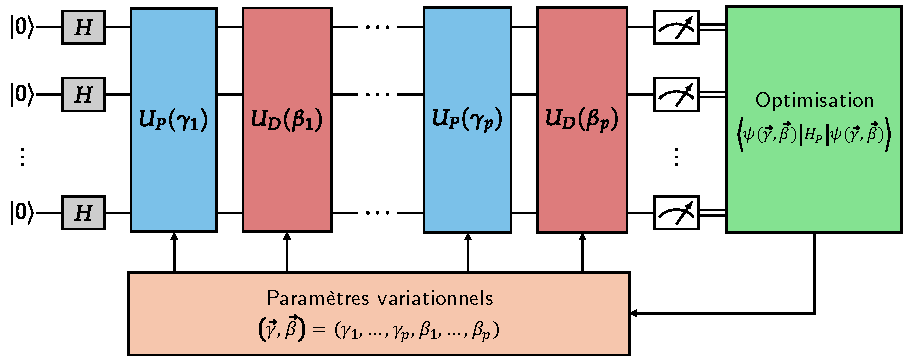
\includegraphics[width=0.9\textwidth]{figures/qaoa.pdf}
    \caption[Algorithme quantique d'optimisation approximative]{Schéma de l'algorithme quantique d'optimisation approximative (QAOA). Un circuit quantique paramétré est préparé en appliquant une alternance d'opérateurs de problème $U_{P}(\gamma)$ et de forçage $U_{D}(\beta)$ à un état initial $\ket{+}^{\otimes n}$. La valeur moyenne $\braket{ \psi(\vec{\gamma}, \vec{\beta}) | H_{P} | \psi(\vec{\gamma}, \vec{\beta}) }$ de l'Hamiltonien de problème $H_{P}$ est ensuite optimisée en modifiant les paramètres $\vec{\gamma}$ et $\vec{\beta}$ du circuit à l'aide d'un optimiseur classique.}
    \label{fig:qaoa}
\end{figure}

Décrivons maintenant plus en détail les mécanismes derrière QAOA: la préparation de l'état initial, l'encodage du problème dans un hamiltonien de problème ainsi que le choix de l'hamiltonien de forçage. L'initialisation et l'optimisation des paramètres du circuit sont décrites à la section~\ref{subsec:configuration-des-parametres}.

%-----------------------------------------------------------------------------%

\subsubsection{Préparation de l'état initial}
\label{subsec:preparation-de-etat-initial}

Comme QAA, le circuit quantique est initialement préparé dans l'état fondamental de l'hamiltonien de forçage pour garantir le théorème adiabatique. Cependant, la divergence de QAOA du calcul adiabatique implique qu'un autre état initial peut être choisi. Une alternative consiste à utiliser une solution approximative du problème comme état initial~\cite{eggerWarmstartingQuantumOptimization2021}. L'état initial peut aussi être choisi de manière à restreindre l'espace des solutions. Au lieu de l'état initial $\ket{\psi_{0}} = \ket{0}^{\otimes n}$, un espace ne représentant que les solutions faisables du problème peut être préparé, tel qu'exemplifié à la section~\ref{subsec:forcage-de-grover}.

%-----------------------------------------------------------------------------%

\subsubsection{Encodage du problème}
\label{subsec:encodage-probleme}

Comment est-ce qu'un problème d'optimisation combinatoire $\varphi(x)$ peut être encodé par un hamiltonien $H_{P}$? D'abord, les entrées $x$ du problème sont caractérisées par une fonction de coût $C(x)$, pénalisant les configurations selon le nombre de contraintes non respectées. Une entrée optimale est associée à un coût nul, alors qu'une entrée non optimale est associée à un coût positif selon sa proximité avec la solution. Résoudre le problème consiste alors à trouver l'entrée optimale, c'est-à-dire l'entrée $x^{*}$ minimisant la fonction de coût. L'hamiltonien de problème se définit à partir de la fonction de coût tel que
\begin{equation}
    H_{P} \ket{x} = C(x) \ket{x} \,.
\end{equation}
Cette équation implique que l'état fondamental de l'hamiltonien $H_{P}$ encode les solutions au problème donné. QAOA cherche ainsi à préparer l'état fondamental de $H_{P}$ comme il correspond à une superposition des solutions au problème $\varphi$. Le modèle d'Ising est fréquemment utilisé pour fournir un hamiltonien de problème décrivant la fonction de coût $C$. En effet, trouver l'état fondamental d'un modèle d'Ising constitue un problème \textsf{NP}-complet, ce qui signifie qu'il existe alors nécessairement une réduction entre ce problème et les différents problèmes \textsf{NP}-complet. Le modèle d'Ising est donné par
\begin{equation}
    \label{eq:hamiltonien-ising}
    H_P = - \sum_{(i,j) \in E} J_{ij} \sigma_i \sigma_j - \sum_{i \in V} h_i \sigma_i \,,
\end{equation}
où $E$ est l'ensemble d'arêtes, $V$ est l'ensemble de sommets et $\sigma_{i}$ est le spin du site $i$. Les constantes $J$ et $h$ représentent respectivement l'interaction entre deux sites et le champ magnétique externe. Le problème d'optimisation quadratique binaire non contraint (« Quadratic Unconstrained Binary Optimization ») (QUBO) permet aussi d'exprimer les fonctions de coût de manière plus générale, en ne les restreignant pas au modèle d'Ising.

\begin{figure}[h]
    \centering
    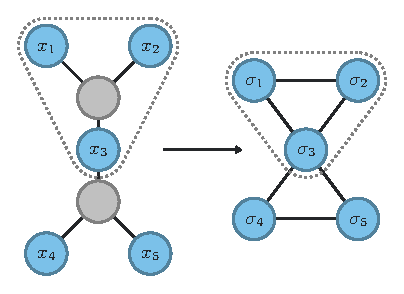
\includegraphics[width=0.6\textwidth]{figures/ising-mapping}
    \caption[Transformation du problème \#NAE3SAT et \#1-in-3SAT au modèle d'Ising]{Exemple de la transformation entre le modèle d'Ising pour NAE3SAT et 1-in-3SAT pour une formule $\varphi$. À gauche, le graphe de facteurs de $\varphi$ avec les sommets de variables (bleus) et de clauses (gris). À droite, le modèle d'Ising correspondant à $\varphi$. Pour 1-in-3SAT, un terme de champ magnétique est ajouté pour favoriser les configurations où chaque clause contient exactement une variable fixée à 1.}
    \label{fig:transformation-ising}
\end{figure}

La formulation de problèmes \textsf{NP}-complet sous la forme du modèle d'Ising n'est pas nécessairement évidente, mais plusieurs réductions ont été formulées pour le calcul adiabatique quantique~\cite{lucasIsingFormulationsMany2014,lodewijksMappingNPhardNPcomplete2020}. Une réduction intéressante dans notre cas relie le problème positif NAE3SAT au modèle d'Ising antiferromagnétique. Une formule CNF $\varphi$ peut être représentée graphiquement sous la forme d'un graphe biparti nommé \textit{graphe de facteurs}. Dans ce graphe, les clauses et les variables forment les deux types de sommets de la bipartition, alors que les arêtes sont définies entre les sommets de ces deux partitions et correspondent à la présence d'une variable dans une clause. Considérons pour le moment une seule clause $C = (x_{1} \lor x_{2} \lor x_{3})$ de $\varphi$ et montrons comment transformer celle-ci au modèle d'Ising. En associant chaque variable $x_{i}$ à un spin $\sigma_{i}$ selon la transformation $\sigma_{i} = 1 - 2x_{i}$, cette clause se réduit à un modèle d'Ising antiferromagnétique en considérant un réseau triangulaire composé des spins $\sigma_{i}$, où chacun de ceux-ci interagit avec les deux autres spins comme illustré à la figure~\ref{fig:transformation-ising}. L'hamiltonien du modèle d'Ising associé à la clause $C = (x_{1} \lor x_{2} \lor x_{3})$ est alors donné par
\begin{equation}
    H_{P, C}^{\text{NAE3SAT}} = \sigma_{1}\sigma_{2} + \sigma_{2}\sigma_{3} + \sigma_{3}\sigma_{1} \,.
\end{equation}
Pour valider cette transformation, l'énergie associée à chaque combinaison possible de spins est présentée dans le tableau~\ref{tab:energie-nae3sat}. La frustration des spins sur le réseau implique que les seuls états qui ne sont pas dans l'état fondamental sont les états $\ket{\uparrow \uparrow \uparrow}$ et $\ket{\downarrow \downarrow \downarrow}$. Or, il s'agit des deux combinaisons ne faisant pas partie de l'ensemble des solutions du problème positif NAE3SAT. L'état fondamental de l'hamiltonien $H_{P, C}$ correspond ainsi bien aux solutions de la clause $C$.

\begin{table}[h]
    \centering
    \begin{subtable}{0.49\textwidth}
        \centering
        \begin{tabular}{c c}
            \hline
            Entrées (spins) & Coût (énergie) \\
            \hline
            000 & 3 \\
            001 & -1 \\
            010 & -1 \\
            100 & -1 \\
            011 & -1 \\
            110 & -1 \\
            101 & -1 \\
            111 & 3 \\
            \hline
        \end{tabular}
        \caption{}
        \label{tab:energie-nae3sat}
    \end{subtable}
    \begin{subtable}{0.49\textwidth}
        \centering
        \begin{tabular}{c c}
            \hline
            Entrées (spins) & Cout (énergie) \\
            \hline
            000 & 0 \\
            001 & -2 \\
            010 & -2 \\
            100 & -2 \\
            011 & 0 \\
            110 & 0 \\
            101 & 0 \\
            111 & 6 \\
            \hline
        \end{tabular}
        \caption{}
        \label{tab:energie-1in3sat}
    \end{subtable}
    \caption{Coût de chaque entrée d'une clause $C = (x_{1} \lor x_{2} \lor x_{3})$ d'une formule CNF pour le problème NAE3SAT (a) et 1-in-3SAT (b). Ce coût correspond à l'énergie du modèle d'Ising donnée par l'hamiltonien $H_{P,C}$ pour une combinaison de spins, reliée aux entrées par la transformation $\sigma_{i} = 1 - 2x_{i}$.}
\end{table}

Une formule CNF est représentable par un modèle d'Ising en appliquant la transformation précédente sur chacune des clauses $C$ de la formule, tel qu'illustré à la figure~\ref{fig:transformation-ising}, donnant ainsi l'hamiltonien 
\begin{equation}
    H_{P} = \sum_{C} H_{P, C} \,.
\end{equation}
Cet hamiltonien impose alors les contraintes de chaque clause. Remarquons que l'hamiltonien de problème pour NAE3SAT est donné par l'hamiltonien d'Ising donné à l'équation~\ref{eq:hamiltonien-ising} avec $J_{ij}=-1$ et $h_{i}=0$ pour un graphe construit comme à la figure~\ref{fig:transformation-ising}. Similairement, le problème 1-in-3SAT se transforme au modèle d'Ising en ajoutant pour chaque clause l'hamiltonien
\begin{equation}
   H_{P, C}^{\text{1-in-3SAT}} = \sigma_{1}\sigma_{2} + \sigma_{2}\sigma_{3} + \sigma_{3}\sigma_{1} - \sigma_{1} - \sigma_{2} - \sigma_{3} \,.
\end{equation}
Un champ magnétique externe est ajouté sur chaque spin pour imposer la contrainte supplémentaire, c'est-à-dire que toutes les clauses doivent contenir exactement une variable évaluant à un vrai logique. Le tableau~\ref{tab:energie-1in3sat} présente les énergies des configurations pour l'hamiltonien précédent, validant la correspondance entre les états fondamentaux et les solutions du problème SAT. L'hamiltonien pour le problème 1-in-3SAT est ainsi donné par l'hamiltonien d'Ising donné à l'équation~\ref{eq:hamiltonien-ising} avec $J_{ij}=-1$ et $h_{i}=1$.

%-----------------------------------------------------------------------------%

\subsubsection{Choix du forçage}

L'hamiltonien de forçage $H_{D}$ initialement proposé avec QAOA prend son inspiration de l'algorithme adiabatique quantique, en utilisant l'hamiltonien facile à préparer $H_{D}^{X}$. Cela implique que toute la dépendance au problème doit être encodée dans l'hamiltonien de problème $H_{P}$. Comme QAOA n'est pas restreint par cette condition, des opportunités se présentent pour encoder différemment le problème. Par exemple, l'hamiltonien de forçage peut être utilisé pour restreindre l'espace de Hilbert en prenant en compte la structure du problème. Divers hamiltoniens offrent différentes performances selon le problème étudié. Le meilleur choix de forçage demeure toutefois une question ouverte.

%-----------------------------------------------------------------------------%

\subsection{Relation avec l'algorithme adiabatique quantique}
\label{subsec:discretisation-qaoa}

QAA requiert une évolution continue de l'état, alors que QAOA repose sur l'application de portes quantiques. Pour établir un lien entre QAA et QAOA, l'évolution de l'hamiltonien de QAA doit donc être rendue discrète. Pour ce faire, l'évolution unitaire de QAA est émulée avec des portes quantiques en décomposant l'opérateur d'évolution $U(t) = e^{-i \int_{0}^{T} H(t) dt}$ de l'hamiltonien de QAA en séquence de petits pas de temps~\cite{blekosReviewQuantumApproximate2024}, tel que
\begin{equation}
    \label{eq:discretisation-qaa}
    U(t) \approx \prod_{k=0}^{t / \Delta t -1} e^{-i H(k \Delta t) \Delta t} \,,
 \end{equation}
pour un intervalle de temps $\Delta t$. Par la suite, la décomposition de Suzuki-Trotter, donnée par $e^{(A+B)t} = \lim_{n \to \infty} (e^{At / n} e^{Bt / n})^{n}$ pour deux opérateurs $A$ et $B$, est employée. Le premier ordre de cette décomposition permet de discrétiser l'opérateur de l'hamiltonien dépendant du temps $H(t)=(1-\frac{t}{T})H_{D} + \frac{t}{T}H_{P}$ de QAA (voir l'équation~\ref{eq:chemin-adiabatique}), où $t \in [0, T]$, tel que
\begin{equation}
    e^{-i H(t) } \approx e^{-i (1 - \frac{t}{T}) H_D \Delta t} e^{-i \frac{t}{T} H_P \Delta t} + O(\Delta t^2) \,.
\end{equation}
La forme de l'opérateur d'évolution de QAOA pour une profondeur $p=1$ de circuit est retrouvée en prenant $\beta = (1 - \frac{t}{T}) \Delta t$ et $\gamma = (\frac{t}{T}) \Delta t$~\cite{sackQuantumAnnealingInitialization2021}. Combinant cette dernière équation avec l'équation~\ref{eq:discretisation-qaa}, l'opérateur d'évolution devient
\begin{equation}
    U(t) \approx \prod_{k=0}^{t / \Delta t -1} e^{-i (1 - \frac{k \Delta t}{T}) H_{D} \Delta t} e^{- i \frac{k \Delta t}{T} H_{P} \Delta t} \,.
 \end{equation}

 Ce processus est généralement nommé \textit{évolution adiabatique trottérisée} en référence à la décomposition de Suzuki-Trotter. Dans la limite $p \to \infty$, une évolution adiabatique est retrouvée, car la condition adiabatique est satisfaite. Pour un circuit de profondeur $p$ finie, plus les paramètres $\gamma$ et $\beta$ sont faibles, plus les erreurs découlant de la discrétisation, communément appelées \textit{erreurs de Trotter}, sont atténuées, car le pas de temps d'évolution est raccourci. Cependant, cela diminue aussi la durée totale d'évolution adiabatique $T$, augmentant ainsi l'impact des excitations diabatiques qui nuisent à la performance de l'algorithme. Au contraire, des paramètres plus grands allongent le temps d'évolution aux dépens de l'augmentation des erreurs de Trotter. Un compromis entre ces deux facteurs doit être choisi pour minimiser les erreurs.

%-----------------------------------------------------------------------------%

\section{Ansatz quantique à opérateurs alternants}
\label{sec:ansatz-quantique-a-operateurs-alternants}

L'algorithme quantique d'optimisation approximative applique en alternance des opérateurs basés sur l'hamiltonien de problème et l'hamiltonien de forçage, guidé par l'algorithme quantique adiabatique. Cet algorithme comporte une limitation importante: les opérateurs appliqués doivent prendre la forme d'une évolution temporelle d'un hamiltonien local fixe. Cette restriction entrave la construction d'opérateurs unitaires potentiellement plus efficaces.

L'\textit{ansatz quantique à opérateurs alternants} (« Quantum Alternating Operator Ansatz») (QAOA), introduit par Hadfield et coll.~\cite{hadfieldQuantumApproximateOptimization2019}, généralise l'algorithme quantique d'optimisation approximative en permettant l'alternance de familles générales d'opérateurs unitaires paramétrés plutôt qu'uniquement des opérateurs basés sur un hamiltonien. Notons qu'un \textit{ansatz} décrit typiquement une sous-routine composée d'une séquence de portes appliquées sur des qubits spécifiques. Cette approche supporte ainsi la représentation d'un plus grand nombre d'états, pouvant possiblement être construite de manière plus efficace. De plus, celle-ci facilite l'utilisation d'opérateurs plus facilement réalisables sur le matériel informatique quantique actuel. Cette extension trouve toutefois son utilité principale dans la création d'opérateurs de forçage. En effet, ces opérateurs peuvent désormais être construit de manière à restreindre l'espace des configurations d'un problème selon ses contraintes et ainsi éviter une recherche de l'espace de Hilbert complet. 

L'algorithme quantique d'optimisation approximative et l'ansatz quantique à opérateurs alternants possèdent le même acronyme. Comme cette dernière étend le premier, l'acronyme QAOA fera référence à l'ansatz quantique à opérateurs alternants pour le reste de la présente section.

%-----------------------------------------------------------------------------%

\subsection{Description de l'approche}

Soit un problème d'optimisation combinatoire $\varphi(x)$ et une fonction de coût $C(x)$ décrivant la qualité des entrées $x$ de $\varphi$. Généralisant l'algorithme de Farhi, Goldstone et Gutmann, QAOA est constitué de deux familles d'opérateurs: les opérateurs de séparation de phase $U_{P}(\gamma)$ et les opérateurs de forçage $U_{D}(\beta)$, où $\gamma$ et $\beta$ sont des paramètres réels. Notons que $U_{P}$ et $U_{D}$ ne sont pas restreints à la classe d'opérateurs $e^{-i \theta H}$. Le circuit QAOA est construit en appliquant en alternance $p$ couches d'opérateurs des deux familles précédentes à un état initial donné.
        
Plutôt que de prendre en compte l'espace de Hilbert complet, un \textit{sous-espace faisable} $F$ est considéré. Cet espace ne représente qu'un sous-ensemble de l'espace des configurations possibles, où seules les configurations respectant les contraintes du problème sont présentes. La restriction provient de la famille d'opérateurs de forçage encodant les différentes contraintes du problème $\varphi$. En général, l'état initial est construit à partir d'une solution faisable alors que l'opérateur de forçage s'assure de restreindre les états possibles au sous-espace faisable. QAOA est donc particulièrement utile pour les problèmes comportant des contraintes rigides. Par exemple, le problème de recouvrement de sommets maximal nécessite que les solutions prennent la forme d'un état de Dicke, c'est-à-dire une superposition de tous les états de même poids d'Hamming. Intuitivement, limiter l'espace des configurations devrait améliorer la performance de l'algorithme. 

Quelques restrictions sont appliquées dans la conception des composantes de QAOA. D'abord, l'état initial doit être trivial à réaliser, c'est-à-dire réalisable avec un circuit de profondeur constante. Les unitaires de séparation de phases doivent être diagonales dans la base computationnelle et sont prises dans la majorité des cas comme $U_{P}(\gamma) = e^{-i \gamma H_{P}}$. La construction des unitaires de forçage est ici d'un plus grand intérêt. Ceux-ci doivent préserver le sous-espace faisable et donc transformer les états faisables en états faisables. Les unitaires de forçage doivent aussi fournir des transitions entre toutes les paires d'états correspondant aux états faisables.

%-----------------------------------------------------------------------------%

\subsection{Forçage de Grover}
\label{subsec:forcage-de-grover}

\textit{L'ansatz quantique à opérateurs alternants avec forçage de Grover} (« Grover-Mixer Quantum Alternating Operator Ansatz ») (GM-QAOA) fut proposé par Bärtschi et Eidenbenz~\cite{bartschiGroverMixersQAOA2020} pour déplacer la complexité de la conception de l'opérateur de forçage à la préparation de l'état initial en s'inspirant de l'algorithme de Grover. Cet algorithme se base sur le cadre théorique défini dans la section précédente pour produire efficacement une superposition égale de toutes les solutions faisables.

Décrivons d'abord rapidement le circuit GM-QAOA, tel qu'illustré à la figure~\ref{fig:gm-qaoa}. Un opérateur unitaire de préparation d'état $U_{S}$ crée une superposition égale $\ket{F}$ de toutes les solutions faisables du sous-espace faisable $F$. Par la suite, similairement à QAOA, les opérateurs unitaires de problème $U_{P}$ et de forçage $U_{M}$ sont appliqués en alternance $p$ fois.

\begin{figure}[ht!]
    \centering
    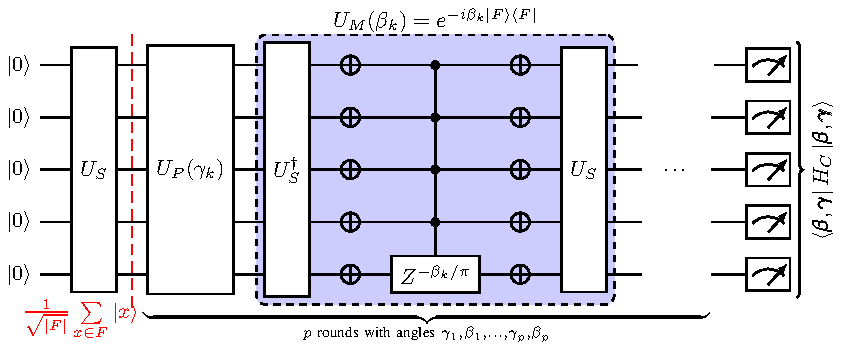
\includegraphics[width=0.7\textwidth]{figures/gm-qaoa}
    \caption[Circuit de l'ansatz quantique à opérateurs alternants avec forçage de Grover]{Première couche du circuit de l'ansatz quantique à opérateurs alternants (GM-QAOA). Ce circuit est composé de l'opérateur de préparation d'état $U_{S}$, de l'opérateur de problème $U_{P}$, de portes de Pauli $X$ ainsi que d'une porte de déphasage $Z^{-\beta \pi}$ contrôlée sur tous les qubits. L'opérateur de forçage $U_{D}$ regroupe les opérateurs à l'intérieur de la boite pointillée.}
    \label{fig:gm-qaoa}
\end{figure}

Plutôt que de préparer un état initial à partir d'un état faisable, comme QAOA, l'état initial de GM-QAOA est préparé dans une superposition de l'entièreté des états faisables. Cette distinction entraine une perspective différente de celle adoptée par QAOA. La difficulté provient désormais de la préparation de l'état plutôt que de la conception de l'opérateur de mélange. L'opérateur de mélange $U_{D}$ quant à lui, est donné par
\begin{equation}
    U_D^{\mathrm{Grover}} = e^{-i \beta \ket{F}\!\bra{F}} = U_{S}\left[ \mathds{1}^{\otimes n} -\left(1-e^{-i \beta}\right) (\ket{0}\!\bra{0})^{\otimes n} \right] U_{S}^{\dagger} \,,
\end{equation}
où $U_{S}$ est l'opérateur de préparation d'état préparant l'état initial $\ket{F}$. L'opérateur $U_{D}^{\mathrm{Grover}}$ s'apparente aux opérateurs de diffusion utilisés dans l'algorithme d'amplification d'amplitude, où les opérateurs de déphasage $e^{-i\beta}$ remplacent les opérateurs d'inversion de phase $e^{-i \pi}$. $U_{D}$ est alors réalisé en utilisant les unitaires $U_{S}$ et $U_{S}^{\dagger}$, deux couches d'opérateur de Pauli $X$ et un opérateur de déphasage $Z^{-\beta/\pi} = \begin{pmatrix}
1 & 0 \\
0 & e^{-i\beta}
\end{pmatrix}$ contrôlés sur tous les qubits.

L'influence de l'algorithme de Grover sur GM-QAOA a notamment pour conséquence que GM-QAOA génère des superpositions uniformes d'états ayant la même énergie. Cette propriété est d'un intérêt particulier pour ce projet, comme elle garantit la distribution de solutions uniforme nécessaire à l'algorithme de JVV. De plus, comme cette approche est réalisable directement à partir d'un ensemble de portes quantiques standard, aucune erreur de simulation d'hamiltonien, comme les erreurs de Trotter, affecte l'algorithme. Notons que les problèmes NAE3SAT et 1-in-3SAT ne sont pas contraints et donc que l'espace faisable demeure le même que pour QAOA, c'est-à-dire que $\ket{F} = \ket{+}^{\otimes n}$.

%-----------------------------------------------------------------------------%

\section{Configuration des paramètres}
\label{subsec:configuration-des-parametres}

La capacité d'entraînement des réseaux de neurones à partir d'une simple descente de gradient fut en partie à l'origine de leur succès retentissant sur de nombreux différents problèmes. L'optimisation des paramètres se fait simplement, même avec des fonctions de coût non convexes, tout en offrant de puissants résultats. Une des attentes envers les VQA était qu'ils possèdent ce même comportement et qu'ils puissent ainsi repousser les limites des algorithmes variationnels. En effet, l'optimisation classique des paramètres de QAOA fait partie intégrante du concept d'algorithme variationnel quantique. Grâce à celle-ci, il est en théorie possible de tirer avantage des algorithmes quantiques en recourant à des ordinateurs quantiques bruités. Cependant, de nombreuses embûches rendent actuellement cette tâche difficile. 

D'abord, l'estimation du gradient de coût est difficile dans de nombreuses situations en raison de la présence de plateaux stériles~\cite{mccleanBarrenPlateausQuantum2018, laroccaReviewBarrenPlateaus2024}, où le gradient devient exponentiellement petit avec la taille du système. Un nombre exponentiel de mesures devient alors nécessaire pour pouvoir identifier la direction minimisant la fonction de coût. Ces complications se présentent surtout pour des circuits de grande profondeur, mais d'autres problèmes surgissent même pour ceux de petites tailles. Un grand nombre de minima locaux sont effectivement considérés comme pauvres, c'est-à-dire qu'ils possèdent une énergie petite par rapport au minimum global, augmentant la difficulté d'atteindre une solution approximative de bonne qualité~\cite{anschuetzQuantumVariationalAlgorithms2022}. De plus, l'optimisation des paramètres des VQA est \textsf{NP}-difficile, et donc intraitable dans le pire des cas~\cite{bittelTrainingVariationalQuantum2021}. Ces difficultés sont d'autant plus importantes comme la complexité de l'espace des paramètres augmente avec le nombre de paramètres d'un circuit, ce qui implique une plus grande difficulté d'optimisation pour les circuits profonds. 

Cet ensemble de complications implique alors qu'une bonne initialisation des paramètres est nécessaire au succès de QAOA. Des paramètres initiaux suffisamment près de l'extremum global peuvent aider à contourner les problèmes énoncés précédemment. Le choix de bons paramètres demeure toutefois une question ouverte. Parmi les différentes approches, Sack et Serbyn proposent une stratégie d'initialisation basée sur le \textit{recuit quantique trottérisé} (« Trotterized Quantum Annealing ») (TQA)~\cite{sackQuantumAnnealingInitialization2021}. Cette méthode, utilisée pour les simulations de ce travail, offre la même performance qu'un nombre exponentiel d'initialisations aléatoires. Comme vu à la section~\ref{subsec:discretisation-qaoa}, un juste milieu doit être choisi entre le temps d'évolution et les erreurs de Trotter. L'initialisation TQA permet de trouver le temps d'évolution optimal à une profondeur de circuit $p$ fixe. Pour ce faire, la procédure décrite à la section~\ref{subsec:discretisation-qaoa} est appliquée sur une grille uniformément discrétisée des temps d'évolution $t_{k} = k \Delta t$, avec $k = 1,\dots, p$, pour un pas de temps $\Delta t = T / p$. Les angles du circuit QAOA correspondant sont alors:
\begin{equation}
    \gamma_{i} = \frac{i}{p} \Delta t \,, \beta = (1 - \frac{i}{p}) \Delta t \,.
\end{equation}
Le pas de temps est optimisé classiquement en mesurant la valeur moyenne de l'hamiltonien de problème $H_{P}$ de manière à minimiser cette dernière, donnant ainsi de bons paramètres initiaux.

%-----------------------------------------------------------------------------%

\section{Échantillonnage et biais}
\label{sec:echantillonnage-et-biais}

L'allure de la distribution obtenue par QAOA est dans notre cas essentiel. Afin de se conformer à la condition de l'algorithme de JVV, celle-ci doit être quasi uniforme, c'est-à-dire qu'elle doit posséder une faible non-uniformité. Est-ce le cas? D'abord, à moins que l'état préparé soit optimal, des non-solutions sont nécessairement présentes dans la distribution obtenue, bien que potentiellement avec une faible probabilité. Comme l'algorithme de JVV nécessite une distribution constituée uniquement de solutions, cela pose problème. Une étape de post-sélection est alors nécessaire pour retirer les non-solutions des échantillons mesurés. Heureusement, vérifier la validité d'une entrée se fait efficacement pour les problèmes \textsf{NP}. Toutefois, rien ne nous garantit que la distribution restante, composée uniquement de solutions, est effectivement non-uniforme.

En général, le recuit quantique n'échantillonne pas les états fondamentaux uniformément~\cite{matsudaGroundstateStatisticsAnnealing2009, mandraExponentiallyBiasedGroundState2017}. Certains états sont exponentiellement supprimés et nécessitent un nombre exponentiel de mesures pour être détectés. Comme le recuit quantique et QAOA sont fortement liés, il est ainsi peu probable que QAOA puisse échantillonner les états fondamentaux de manière uniforme.

Une propriété de l'algorithme GM-QAOA devient alors d'un intérêt considérable: l'équiprobabilité des états de même énergie. Les solutions étant encodées dans l'état fondamental de l'hamiltonien de problème, elles possèdent ainsi la même amplitude et donc la même probabilité. En ne considérant que les solutions, l'état préparé par le circuit GM-QAOA possède toujours une non-uniformité nulle, un avantage non négligeable par rapport à QAOA.
